\chapter{Recolección de Datos}\label{chap:recoleccion}

El presente capitulo es de gran importancia para el desarrollo de esta investigación ya que se describe como se llevo a cabo la recolección de los datos necesarios para alcanzar los objetivos planteados. Se presenta al lector los diversos pasos para la obtención de las imágenes, ademas de las diversas configuraciones realizadas para la ejecución de los experimentos.

\section{Imágenes Satelitales}\label{sec:imagen_satelitales}

Una imagen satelital se la puede definir como la representación visual de información capturada por un sensor montado en un satélite artificial. Estos sensores recogen la información reflejada por la superficie de la tierra que luego es enviada para su posterior procesamiento.

El uso de imágenes satelitales constituye una excelente herramienta para el conocimiento y monitoreo de los territorios y recursos; hoy en día disfrutamos de la oportunidad de aprovechar de imágenes satelitales para una gran variedad de aplicaciones:
\begin{itemize}
	\item Desarrollo y planificación urbana.
	\item Infraestructura, carreteras, canales, tuberías etc.
	\item Recursos naturales.
	\item Investigación.
	\item Alerta temprana de catástrofes.
	\item Asuntos militares.
	\item entre otras aplicaciones.
\end{itemize}

\subsection{Niveles de procesamiento}\label{sub:nivelesdeprocesamiento}
Dependiendo de la agencia espacial existe una nomenclatura para determinar los niveles de procesamiento que se aplica a las imágenes satelitales. En nuestro caso vamos a utilizar las siguiente nomenclatura impuesta por la \ac{nasa}:
\begin{itemize}
	\item \textbf{Nivel 0}: La información científica recogida está a máxima resolución, ordenada temporalmente y con errores de transmisión, artefactos y duplicados eliminados.
 	\item \textbf{Nivel 1a}: La información esta ordenada cronológicamente y datos auxiliares como coeficientes de calibración y parámetros de referencia.
 	\item \textbf{Nivel 1b}: La información del 1a es procesada a unidades de detección, geo-refereciada.
 	\item \textbf{Nivel 2}: Variables geofísicas derivadas por ejemplo productos de concentraciones de hielo, ola de mar, etc.
 	\item \textbf{Nivel 3}: Las variables son mapeadas uniformemente en \textit{grids} espacio-temporales.
 	\item \textbf{Nivel 4}: Resultados de los análisis de los niveles anteriores
\end{itemize}


\section{Datos utilizdos}\label{sec:datosutilizados}

En base a lo mencionado en la sección \ref{sec:funcamentacion}, las imágenes que se utilizaron para el desarrollo de esta tesis fueron seleccionadas a partir de los requerimientos impuesto por el \ac{FS} \ac{conae}. Estas imágenes se asemejan a la cámara que será utilizada en el proyecto mencionado anteriormente. Las imágenes escogidas que se asemejan a las características impuestas por los requerimientos expuestos fueron adquiridas por el instrumento \ac{viirs} a bordo del satélite Suomi-NPP \ref{sub:viirs}.

Las imágenes fueron descargadas por medio del catalogo  publicado en el sitio oficial de \ac{conae} \footnote{Fuente: http://catalogos.conae.gov.ar/catalogo/catalogo-de-imagenes.html} de acceso gratuito para el publico. Se debe señalar ademas que se trabajó con imágenes correspondiente a los años 2017 y 2018 en una ventana de tiempo desde Abril del 2017 a Marzo del 2018; estas imágenes son de naturaleza óptica con un nivel de procesamiento 1a, de acuerdo a las nomenclaturas utilizadas en la sección \ref{sub:nivelesdeprocesamiento}.



\subsection{VIIRS}\label{sub:viirs}
El instrumento \ac{viirs} fue lanzado a bordo del satélite Suomi-NPP el 28 de octubre de 2011. Este instrumento posee 5 canales de alta resolución (I-bands), 16 canales de resolución moderada (M-bands) y un canal de baja luz (Day/Night Band, DNB). 

En el siguiente cuadro se detallan las diferentes longitudes de onda y los rangos de onda de las bandas, junto con resolución geométrica apuntando a Nadir (ver tabla: \ref{tab:viirs}).
\begin{table}[H]
\begin{center}
\begin{tabular}{|c|c|c|}
\hline Banda & Rango Espectral (um) & Resolución Nadir \\\hline 
 		M1  & 0.402-0.422   & 0.742 x 0.259 \\ \hline 
		M2  & 0.436-0.454   & 0.742 x 0.259 \\ \hline 
		M3  & 0.478-0.498   & 0.742 x 0.259 \\ \hline 
		M4  & 0.545-0.565   & 0.742 x 0.259 \\ \hline 
		I1  & 0.600-0.680   & 0.371 x 0.387 \\ \hline 
		M5  & 0.662-0.682   & 0.742 x 0.259 \\ \hline 
		M6  & 0.739-0.754   & 0.742 x 0.776 \\ \hline 
		I2  & 0.846-0.885   & 0.371 x 0.387 \\ \hline 
		M7  & 0.846-0.885   & 0.742 x 0.259 \\ \hline 
		M8  & 1.230-1.250   & 0.742 x 0.776 \\ \hline 
		M9  & 1.371-1.386   & 0.742 x 0.776 \\ \hline 
		I3  & 1.580-1.640   & 0.371 x 0.387 \\ \hline 
		M10 & 1.580-1.640   & 0.742 x 0.776 \\ \hline 
		M11 & 2.225-2.275   & 0.742 x 0.776 \\ \hline 
		I4  & 3.550-3.930   & 0.371 x 0.387 \\ \hline 
		M12 & 3.660-3.840   & 0.742 x 0.776 \\ \hline 
		M13 & 3.973-4.128   & 0.742 x 0.259 \\ \hline 
		M14 & 8.400-8.700   & 0.742 x 0.776 \\ \hline 
		M15 & 10.263-11.263 & 0.742 x 0.776 \\ \hline 
		I5  & 10.500-12.400 & 0.371 x 0.387 \\ \hline 
		M16 & 11.538-12.488 & 0.742 x 0.776 \\ \hline 
\end{tabular}
\end{center}\caption{Característica de bandas,\ac{viirs} \label{tab:viirs}}
\end{table}


En la siguiente figura \ref{Fig: bandas543} podemos visualizar unas de las características de utilizadas; en este caso una imagen correspondiente a la combinaciones de bandas M5, M4, M3 conocidas como (\textit{True Color}), color verdadero.

\begin{figure}[H]
 \centering
  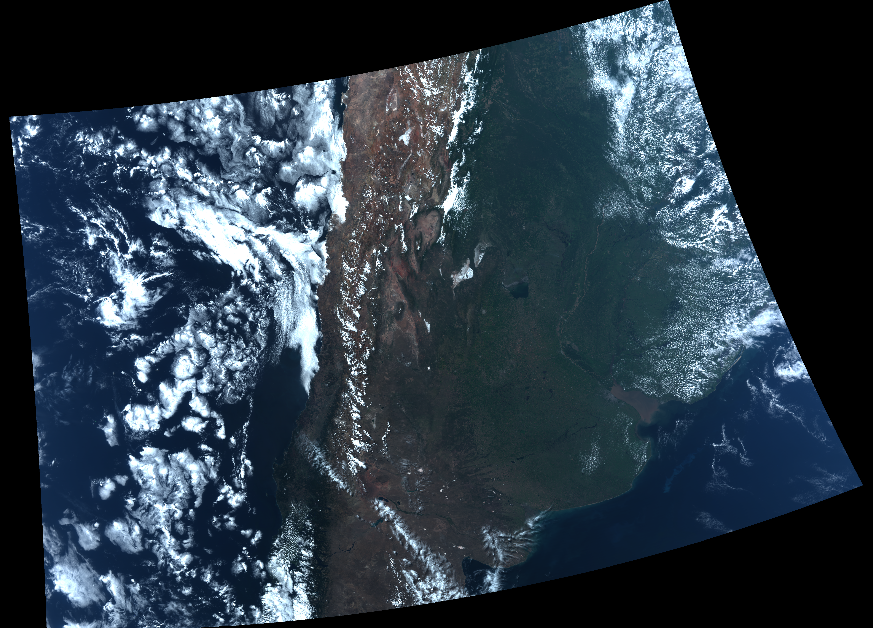
\includegraphics[height=10cm,keepaspectratio=true,clip=true]{imagenes/RecolecciondeDatos/img-543.png}
  \caption{Combinación de bandas M5, M4 y M3, Suomi-NPP}
	\label{Fig: bandas543}
\end{figure}


\subsection{Combinaciones de Bandas}\label{sub:comb_de_banda}

Las bandas  utilizadas para este trabajo de tesis  son las  de resolución moderada (M-bands) vistas en \ref{tab:viirs} , que posee una resolución espacial a nadir de 750 metros.

En el siguiente cuadro se detalla las diferentes combinaciones de bandas utilizadas para este trabajo.


% ACA FALTA PONER TODAS LAS BANDAS QUE SE USO EN EL TRABAJO
\begin{table}[H] \begin{center}
\begin{tabular}{c|c}
Num & Combinación de banda\\ \hline 
		1  & a \\ 					 \hline
		2  & a \\ 					 \hline
    	3  & a \\ 					 \hline
		4  & a \\ 					 \hline
		5  & a \\ 					 \hline
    	6  & a \\ 					 \hline
		7  & a \\ 					 \hline
		8  & a \\ 					 \hline
    	9  & a \\ 					 \hline
		10 & a \\ 					 \hline
		11 & a \\ 					 \hline
    	12 & a \\ 					 \hline
		13 & a \\ 					 \hline
		14 & a \\ 					 \hline
    	15 & a \\ 					 \hline
		16 & a \\ 					 \hline
		17 & a \\ 					 \hline
    	18 & a \\ 					 \hline
		19 & a \\ 					 \hline
		20 & a \\ 					 \hline
    	21 & a \\ 					 \hline    	
\end{tabular}
\end{center}\caption{Combinaciones de bandas utilizadas \label{tab:combinacion_banda}}
\end{table}
\section{Recolección de Imágenes}\label{sub:recolecciondeimagen}

Para recolectar las imágenes mencionadas en la sección anterior: \ref{sub:datosutilizados}, se debió realizar diversos pasos para obtener una imagen que luego serán utilizadas en los experimentos. Los pasos que se llevaron a cabo podemos enumerar  en:
\begin{enumerate}
	\item Descarga de imágenes.
	\item Pre-procesamiento.
\end{enumerate}

El primer punto se hace referencia a la descarga manual de los datos por medio del sitio oficial de \ac{conae}; ademas de realizo un pedido para poder obtener una ventana temporal de imágenes mas amplia ya que en la pagina oficial solo están imágenes que poseen una ventana de tiempo de dos meses.

El segundo y ultimo punto es el que llamamos pre-procesamiento, en el las tareas que se realizaron fueron para obtener la imagen final a ser utilizada para la investigación.
Partiendo de la imagen obtenida en el punto uno se utilizo la herramienta de procesamiento de imágenes ENVI \ref{sub:enviSoft}, software para el análisis de imágenes. Este software nos proporciona diferentes herramientas para la manipulación y procesamiento  de  una imagen satelital, de las cuales podemos mencionar la \textit{VIIRS Conversion Toolkit}; herramienta nos permite trabajar con productos \ac{viirs}, pudiendo aplicar a las imágenes correcciones geométricas, geo-referenciacion y re-proyecciones entre las diferentes funcionalidades que nos brinda. En este proceso de conversión de imágenes se realizaron diversos pasos para la obtención de las imágenes finales. Los pasos llevados a cabos a través del sofware \textit{ENVI} fueron los siguientes:

\begin{enumerate}

\item Inicio, pantalla principal ENVI:
	\begin{figure}[H]\centering
		
\includegraphics[height=1.5cm,keepaspectratio=true,clip=true]{imagenes/RecolecciondeDatos/envi1.png}
  		\caption{Pantalla Principal ENVI} \label{Fig: envi1}
	\end{figure}


\item Procesamiento: abrir la herramienta \textit{VIIRS Conversion Toolkit} e ingresar los archivos de cada banda adjuntando el archivo  geo-referenciado, para realizar la carga de la imagen manual(figura: \ref{Fig: envi2}).

\begin{figure}[H] \centering
  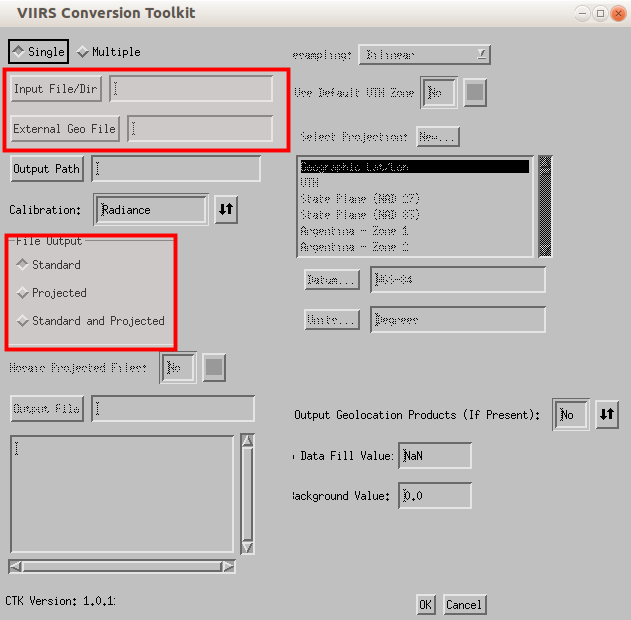
\includegraphics[height=9cm,keepaspectratio=true,clip=true]{imagenes/RecolecciondeDatos/envi2.png}
  \caption{Cargar Bandas ENVI Toolkit} \label{Fig: envi2}
\end{figure}

\item Re-proyección de imagen: adjuntar bandas a utilizar; se debe asignar de acuerdo al color que corresponda cada banda (RGB) (figura: \ref{Fig: envi3}).
 
\begin{figure}[H]
 \centering
  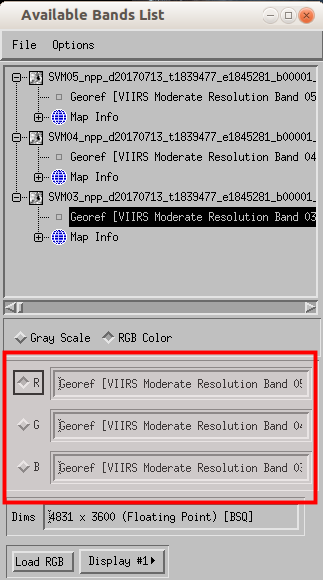
\includegraphics[height=9cm,keepaspectratio=true,clip=true]{imagenes/RecolecciondeDatos/envi3.png}
  \caption{Ejemplo re-proyección \textit{True Color}}
	\label{Fig: envi3}
\end{figure}

\end{enumerate}


Cada imagen obtenida a partir del proceso mencionado anteriormente se almaceno en formato \textit{.tiff} para su posterior procesamiento de experimentos.